\documentclass[11pt,a4paper]{article}

% shared/macros.tex
% Shared notation for all surface-partition math documents.
% Include with: % shared/macros.tex
% Shared notation for all surface-partition math documents.
% Include with: % shared/macros.tex
% Shared notation for all surface-partition math documents.
% Include with: \input{../shared/macros}

% -------------------------------------------------------------------------
% Packages (include here so each document only needs \input{../shared/macros})
% -------------------------------------------------------------------------
\usepackage{amsmath,amssymb,amsthm}
\usepackage{bm}           % \bm for bold math
\usepackage{mathtools}    % \coloneqq, dcases, etc.
\usepackage{booktabs}     % \toprule etc. in tables
\usepackage{hyperref}
\usepackage{geometry}
\usepackage{microtype}
\usepackage{parskip}
\usepackage{xcolor}
\usepackage{tcolorbox}
\usepackage{enumitem}
\usepackage{float}             % [H] float placement

\geometry{a4paper, margin=2.5cm}

% -------------------------------------------------------------------------
% Theorem-like environments
% -------------------------------------------------------------------------
\theoremstyle{definition}
\newtheorem{defn}{Definition}[section]
\newtheorem{remark}{Remark}[section]

\theoremstyle{plain}
\newtheorem{prop}{Proposition}[section]

% -------------------------------------------------------------------------
% Mesh and geometry
% -------------------------------------------------------------------------
\newcommand{\V}{\mathbf{V}}            % vertex array V[i] in R^dim
\newcommand{\F}{\mathbf{F}}            % face (triangle) array
\newcommand{\vone}[1]{v_{1,#1}}       % first vertex index of VP i
\newcommand{\vtwo}[1]{v_{2,#1}}       % second vertex index of VP i

% -------------------------------------------------------------------------
% Variable points
% -------------------------------------------------------------------------
\newcommand{\lam}{\lambda}             % scalar VP parameter
\newcommand{\Lam}{\boldsymbol{\lambda}}% full parameter vector
\newcommand{\vp}[1]{\mathbf{p}_{#1}}  % 3D position of VP i
\newcommand{\ed}[1]{\mathbf{d}_{#1}}  % edge direction d_i = V[v1_i] - V[v2_i]

% -------------------------------------------------------------------------
% Steiner / triple-point
% -------------------------------------------------------------------------
\newcommand{\Sv}{\mathbf{S}}           % Steiner (Fermat-Torricelli) point
\newcommand{\Ki}{K_{i}}               % projection matrix (I-n_i n_i^T)/r_i
\newcommand{\Mmat}{M}                 % sum of K_i matrices at a triple point

% -------------------------------------------------------------------------
% Normals and unit vectors
% -------------------------------------------------------------------------
\newcommand{\nhat}{\hat{\mathbf{n}}}  % unit normal to a triangle
\newcommand{\Dhat}{\hat{\boldsymbol{\Delta}}}  % unit segment direction

% -------------------------------------------------------------------------
% Operations
% -------------------------------------------------------------------------
\newcommand{\norm}[1]{\left\|#1\right\|}
\newcommand{\abs}[1]{\left|#1\right|}
\newcommand{\ip}[2]{\langle #1,\, #2 \rangle}

% Projection perpendicular to a unit vector \uhat
\newcommand{\Proj}[1]{\bigl(\mathbf{I} - #1 #1^\top\bigr)}

% argmax operator (winner-take-all assignment in Phase 1 documents)
\DeclareMathOperator*{\argmax}{arg\,max}
\DeclareMathOperator*{\argmin}{arg\,min}

% -------------------------------------------------------------------------
% Calculus shorthands
% -------------------------------------------------------------------------
\newcommand{\pd}[2]{\dfrac{\partial #1}{\partial #2}}
\newcommand{\pdd}[3]{\dfrac{\partial^2 #1}{\partial #2\,\partial #3}}
\newcommand{\grad}{\nabla}
\newcommand{\Hess}[1]{\nabla^2 #1}

% -------------------------------------------------------------------------
% Optimization problem objects
% -------------------------------------------------------------------------
\newcommand{\Preg}{P_{\mathrm{reg}}}  % regular perimeter
\newcommand{\Pst}{P_{\mathrm{st}}}   % Steiner perimeter
\newcommand{\Areg}{A^{\mathrm{reg}}} % regular cell area
\newcommand{\Ast}{A^{\mathrm{st}}}   % Steiner area contribution
\newcommand{\Atgt}{\bar{A}}           % target area per cell
\newcommand{\Lagr}{\mathcal{L}}       % Lagrangian
\newcommand{\objfac}{\sigma}          % IPOPT objective scaling factor

% -------------------------------------------------------------------------
% Code cross-references (for "In the code..." callouts)
% -------------------------------------------------------------------------
\newcommand{\code}[1]{\texttt{#1}}
\newcommand{\codefile}[1]{\texttt{\small #1}}

% -------------------------------------------------------------------------
% Threshold dynamics / approach B (10-mbo-auction-dynamics)
% -------------------------------------------------------------------------
\newcommand{\Dlump}{D}                 % lumped mass matrix diag(v)
\newcommand{\Atau}{A_\tau}             % discrete diffusion operator (M + tau K)^{-1} M
\newcommand{\Etau}{E_\tau}             % heat-content (threshold-dynamics) energy
\newcommand{\Rcell}{R_{\mathrm{cell}}} % radius of the equal-area disc sqrt(Abar/pi)
\newcommand{\hmean}{h_{\mathrm{mean}}} % mean edge length
\newcommand{\hmax}{h_{\mathrm{max}}}   % max edge length
\newcommand{\Gt}{G_t}                  % heat kernel at time t
\newcommand{\Ktau}{K^{\mathrm{res}}_\tau} % resolvent (backward-Euler) kernel


% -------------------------------------------------------------------------
% Packages (include here so each document only needs % shared/macros.tex
% Shared notation for all surface-partition math documents.
% Include with: \input{../shared/macros}

% -------------------------------------------------------------------------
% Packages (include here so each document only needs \input{../shared/macros})
% -------------------------------------------------------------------------
\usepackage{amsmath,amssymb,amsthm}
\usepackage{bm}           % \bm for bold math
\usepackage{mathtools}    % \coloneqq, dcases, etc.
\usepackage{booktabs}     % \toprule etc. in tables
\usepackage{hyperref}
\usepackage{geometry}
\usepackage{microtype}
\usepackage{parskip}
\usepackage{xcolor}
\usepackage{tcolorbox}
\usepackage{enumitem}
\usepackage{float}             % [H] float placement

\geometry{a4paper, margin=2.5cm}

% -------------------------------------------------------------------------
% Theorem-like environments
% -------------------------------------------------------------------------
\theoremstyle{definition}
\newtheorem{defn}{Definition}[section]
\newtheorem{remark}{Remark}[section]

\theoremstyle{plain}
\newtheorem{prop}{Proposition}[section]

% -------------------------------------------------------------------------
% Mesh and geometry
% -------------------------------------------------------------------------
\newcommand{\V}{\mathbf{V}}            % vertex array V[i] in R^dim
\newcommand{\F}{\mathbf{F}}            % face (triangle) array
\newcommand{\vone}[1]{v_{1,#1}}       % first vertex index of VP i
\newcommand{\vtwo}[1]{v_{2,#1}}       % second vertex index of VP i

% -------------------------------------------------------------------------
% Variable points
% -------------------------------------------------------------------------
\newcommand{\lam}{\lambda}             % scalar VP parameter
\newcommand{\Lam}{\boldsymbol{\lambda}}% full parameter vector
\newcommand{\vp}[1]{\mathbf{p}_{#1}}  % 3D position of VP i
\newcommand{\ed}[1]{\mathbf{d}_{#1}}  % edge direction d_i = V[v1_i] - V[v2_i]

% -------------------------------------------------------------------------
% Steiner / triple-point
% -------------------------------------------------------------------------
\newcommand{\Sv}{\mathbf{S}}           % Steiner (Fermat-Torricelli) point
\newcommand{\Ki}{K_{i}}               % projection matrix (I-n_i n_i^T)/r_i
\newcommand{\Mmat}{M}                 % sum of K_i matrices at a triple point

% -------------------------------------------------------------------------
% Normals and unit vectors
% -------------------------------------------------------------------------
\newcommand{\nhat}{\hat{\mathbf{n}}}  % unit normal to a triangle
\newcommand{\Dhat}{\hat{\boldsymbol{\Delta}}}  % unit segment direction

% -------------------------------------------------------------------------
% Operations
% -------------------------------------------------------------------------
\newcommand{\norm}[1]{\left\|#1\right\|}
\newcommand{\abs}[1]{\left|#1\right|}
\newcommand{\ip}[2]{\langle #1,\, #2 \rangle}

% Projection perpendicular to a unit vector \uhat
\newcommand{\Proj}[1]{\bigl(\mathbf{I} - #1 #1^\top\bigr)}

% argmax operator (winner-take-all assignment in Phase 1 documents)
\DeclareMathOperator*{\argmax}{arg\,max}
\DeclareMathOperator*{\argmin}{arg\,min}

% -------------------------------------------------------------------------
% Calculus shorthands
% -------------------------------------------------------------------------
\newcommand{\pd}[2]{\dfrac{\partial #1}{\partial #2}}
\newcommand{\pdd}[3]{\dfrac{\partial^2 #1}{\partial #2\,\partial #3}}
\newcommand{\grad}{\nabla}
\newcommand{\Hess}[1]{\nabla^2 #1}

% -------------------------------------------------------------------------
% Optimization problem objects
% -------------------------------------------------------------------------
\newcommand{\Preg}{P_{\mathrm{reg}}}  % regular perimeter
\newcommand{\Pst}{P_{\mathrm{st}}}   % Steiner perimeter
\newcommand{\Areg}{A^{\mathrm{reg}}} % regular cell area
\newcommand{\Ast}{A^{\mathrm{st}}}   % Steiner area contribution
\newcommand{\Atgt}{\bar{A}}           % target area per cell
\newcommand{\Lagr}{\mathcal{L}}       % Lagrangian
\newcommand{\objfac}{\sigma}          % IPOPT objective scaling factor

% -------------------------------------------------------------------------
% Code cross-references (for "In the code..." callouts)
% -------------------------------------------------------------------------
\newcommand{\code}[1]{\texttt{#1}}
\newcommand{\codefile}[1]{\texttt{\small #1}}

% -------------------------------------------------------------------------
% Threshold dynamics / approach B (10-mbo-auction-dynamics)
% -------------------------------------------------------------------------
\newcommand{\Dlump}{D}                 % lumped mass matrix diag(v)
\newcommand{\Atau}{A_\tau}             % discrete diffusion operator (M + tau K)^{-1} M
\newcommand{\Etau}{E_\tau}             % heat-content (threshold-dynamics) energy
\newcommand{\Rcell}{R_{\mathrm{cell}}} % radius of the equal-area disc sqrt(Abar/pi)
\newcommand{\hmean}{h_{\mathrm{mean}}} % mean edge length
\newcommand{\hmax}{h_{\mathrm{max}}}   % max edge length
\newcommand{\Gt}{G_t}                  % heat kernel at time t
\newcommand{\Ktau}{K^{\mathrm{res}}_\tau} % resolvent (backward-Euler) kernel
)
% -------------------------------------------------------------------------
\usepackage{amsmath,amssymb,amsthm}
\usepackage{bm}           % \bm for bold math
\usepackage{mathtools}    % \coloneqq, dcases, etc.
\usepackage{booktabs}     % \toprule etc. in tables
\usepackage{hyperref}
\usepackage{geometry}
\usepackage{microtype}
\usepackage{parskip}
\usepackage{xcolor}
\usepackage{tcolorbox}
\usepackage{enumitem}
\usepackage{float}             % [H] float placement

\geometry{a4paper, margin=2.5cm}

% -------------------------------------------------------------------------
% Theorem-like environments
% -------------------------------------------------------------------------
\theoremstyle{definition}
\newtheorem{defn}{Definition}[section]
\newtheorem{remark}{Remark}[section]

\theoremstyle{plain}
\newtheorem{prop}{Proposition}[section]

% -------------------------------------------------------------------------
% Mesh and geometry
% -------------------------------------------------------------------------
\newcommand{\V}{\mathbf{V}}            % vertex array V[i] in R^dim
\newcommand{\F}{\mathbf{F}}            % face (triangle) array
\newcommand{\vone}[1]{v_{1,#1}}       % first vertex index of VP i
\newcommand{\vtwo}[1]{v_{2,#1}}       % second vertex index of VP i

% -------------------------------------------------------------------------
% Variable points
% -------------------------------------------------------------------------
\newcommand{\lam}{\lambda}             % scalar VP parameter
\newcommand{\Lam}{\boldsymbol{\lambda}}% full parameter vector
\newcommand{\vp}[1]{\mathbf{p}_{#1}}  % 3D position of VP i
\newcommand{\ed}[1]{\mathbf{d}_{#1}}  % edge direction d_i = V[v1_i] - V[v2_i]

% -------------------------------------------------------------------------
% Steiner / triple-point
% -------------------------------------------------------------------------
\newcommand{\Sv}{\mathbf{S}}           % Steiner (Fermat-Torricelli) point
\newcommand{\Ki}{K_{i}}               % projection matrix (I-n_i n_i^T)/r_i
\newcommand{\Mmat}{M}                 % sum of K_i matrices at a triple point

% -------------------------------------------------------------------------
% Normals and unit vectors
% -------------------------------------------------------------------------
\newcommand{\nhat}{\hat{\mathbf{n}}}  % unit normal to a triangle
\newcommand{\Dhat}{\hat{\boldsymbol{\Delta}}}  % unit segment direction

% -------------------------------------------------------------------------
% Operations
% -------------------------------------------------------------------------
\newcommand{\norm}[1]{\left\|#1\right\|}
\newcommand{\abs}[1]{\left|#1\right|}
\newcommand{\ip}[2]{\langle #1,\, #2 \rangle}

% Projection perpendicular to a unit vector \uhat
\newcommand{\Proj}[1]{\bigl(\mathbf{I} - #1 #1^\top\bigr)}

% argmax operator (winner-take-all assignment in Phase 1 documents)
\DeclareMathOperator*{\argmax}{arg\,max}
\DeclareMathOperator*{\argmin}{arg\,min}

% -------------------------------------------------------------------------
% Calculus shorthands
% -------------------------------------------------------------------------
\newcommand{\pd}[2]{\dfrac{\partial #1}{\partial #2}}
\newcommand{\pdd}[3]{\dfrac{\partial^2 #1}{\partial #2\,\partial #3}}
\newcommand{\grad}{\nabla}
\newcommand{\Hess}[1]{\nabla^2 #1}

% -------------------------------------------------------------------------
% Optimization problem objects
% -------------------------------------------------------------------------
\newcommand{\Preg}{P_{\mathrm{reg}}}  % regular perimeter
\newcommand{\Pst}{P_{\mathrm{st}}}   % Steiner perimeter
\newcommand{\Areg}{A^{\mathrm{reg}}} % regular cell area
\newcommand{\Ast}{A^{\mathrm{st}}}   % Steiner area contribution
\newcommand{\Atgt}{\bar{A}}           % target area per cell
\newcommand{\Lagr}{\mathcal{L}}       % Lagrangian
\newcommand{\objfac}{\sigma}          % IPOPT objective scaling factor

% -------------------------------------------------------------------------
% Code cross-references (for "In the code..." callouts)
% -------------------------------------------------------------------------
\newcommand{\code}[1]{\texttt{#1}}
\newcommand{\codefile}[1]{\texttt{\small #1}}

% -------------------------------------------------------------------------
% Threshold dynamics / approach B (10-mbo-auction-dynamics)
% -------------------------------------------------------------------------
\newcommand{\Dlump}{D}                 % lumped mass matrix diag(v)
\newcommand{\Atau}{A_\tau}             % discrete diffusion operator (M + tau K)^{-1} M
\newcommand{\Etau}{E_\tau}             % heat-content (threshold-dynamics) energy
\newcommand{\Rcell}{R_{\mathrm{cell}}} % radius of the equal-area disc sqrt(Abar/pi)
\newcommand{\hmean}{h_{\mathrm{mean}}} % mean edge length
\newcommand{\hmax}{h_{\mathrm{max}}}   % max edge length
\newcommand{\Gt}{G_t}                  % heat kernel at time t
\newcommand{\Ktau}{K^{\mathrm{res}}_\tau} % resolvent (backward-Euler) kernel


% -------------------------------------------------------------------------
% Packages (include here so each document only needs % shared/macros.tex
% Shared notation for all surface-partition math documents.
% Include with: % shared/macros.tex
% Shared notation for all surface-partition math documents.
% Include with: \input{../shared/macros}

% -------------------------------------------------------------------------
% Packages (include here so each document only needs \input{../shared/macros})
% -------------------------------------------------------------------------
\usepackage{amsmath,amssymb,amsthm}
\usepackage{bm}           % \bm for bold math
\usepackage{mathtools}    % \coloneqq, dcases, etc.
\usepackage{booktabs}     % \toprule etc. in tables
\usepackage{hyperref}
\usepackage{geometry}
\usepackage{microtype}
\usepackage{parskip}
\usepackage{xcolor}
\usepackage{tcolorbox}
\usepackage{enumitem}
\usepackage{float}             % [H] float placement

\geometry{a4paper, margin=2.5cm}

% -------------------------------------------------------------------------
% Theorem-like environments
% -------------------------------------------------------------------------
\theoremstyle{definition}
\newtheorem{defn}{Definition}[section]
\newtheorem{remark}{Remark}[section]

\theoremstyle{plain}
\newtheorem{prop}{Proposition}[section]

% -------------------------------------------------------------------------
% Mesh and geometry
% -------------------------------------------------------------------------
\newcommand{\V}{\mathbf{V}}            % vertex array V[i] in R^dim
\newcommand{\F}{\mathbf{F}}            % face (triangle) array
\newcommand{\vone}[1]{v_{1,#1}}       % first vertex index of VP i
\newcommand{\vtwo}[1]{v_{2,#1}}       % second vertex index of VP i

% -------------------------------------------------------------------------
% Variable points
% -------------------------------------------------------------------------
\newcommand{\lam}{\lambda}             % scalar VP parameter
\newcommand{\Lam}{\boldsymbol{\lambda}}% full parameter vector
\newcommand{\vp}[1]{\mathbf{p}_{#1}}  % 3D position of VP i
\newcommand{\ed}[1]{\mathbf{d}_{#1}}  % edge direction d_i = V[v1_i] - V[v2_i]

% -------------------------------------------------------------------------
% Steiner / triple-point
% -------------------------------------------------------------------------
\newcommand{\Sv}{\mathbf{S}}           % Steiner (Fermat-Torricelli) point
\newcommand{\Ki}{K_{i}}               % projection matrix (I-n_i n_i^T)/r_i
\newcommand{\Mmat}{M}                 % sum of K_i matrices at a triple point

% -------------------------------------------------------------------------
% Normals and unit vectors
% -------------------------------------------------------------------------
\newcommand{\nhat}{\hat{\mathbf{n}}}  % unit normal to a triangle
\newcommand{\Dhat}{\hat{\boldsymbol{\Delta}}}  % unit segment direction

% -------------------------------------------------------------------------
% Operations
% -------------------------------------------------------------------------
\newcommand{\norm}[1]{\left\|#1\right\|}
\newcommand{\abs}[1]{\left|#1\right|}
\newcommand{\ip}[2]{\langle #1,\, #2 \rangle}

% Projection perpendicular to a unit vector \uhat
\newcommand{\Proj}[1]{\bigl(\mathbf{I} - #1 #1^\top\bigr)}

% argmax operator (winner-take-all assignment in Phase 1 documents)
\DeclareMathOperator*{\argmax}{arg\,max}
\DeclareMathOperator*{\argmin}{arg\,min}

% -------------------------------------------------------------------------
% Calculus shorthands
% -------------------------------------------------------------------------
\newcommand{\pd}[2]{\dfrac{\partial #1}{\partial #2}}
\newcommand{\pdd}[3]{\dfrac{\partial^2 #1}{\partial #2\,\partial #3}}
\newcommand{\grad}{\nabla}
\newcommand{\Hess}[1]{\nabla^2 #1}

% -------------------------------------------------------------------------
% Optimization problem objects
% -------------------------------------------------------------------------
\newcommand{\Preg}{P_{\mathrm{reg}}}  % regular perimeter
\newcommand{\Pst}{P_{\mathrm{st}}}   % Steiner perimeter
\newcommand{\Areg}{A^{\mathrm{reg}}} % regular cell area
\newcommand{\Ast}{A^{\mathrm{st}}}   % Steiner area contribution
\newcommand{\Atgt}{\bar{A}}           % target area per cell
\newcommand{\Lagr}{\mathcal{L}}       % Lagrangian
\newcommand{\objfac}{\sigma}          % IPOPT objective scaling factor

% -------------------------------------------------------------------------
% Code cross-references (for "In the code..." callouts)
% -------------------------------------------------------------------------
\newcommand{\code}[1]{\texttt{#1}}
\newcommand{\codefile}[1]{\texttt{\small #1}}

% -------------------------------------------------------------------------
% Threshold dynamics / approach B (10-mbo-auction-dynamics)
% -------------------------------------------------------------------------
\newcommand{\Dlump}{D}                 % lumped mass matrix diag(v)
\newcommand{\Atau}{A_\tau}             % discrete diffusion operator (M + tau K)^{-1} M
\newcommand{\Etau}{E_\tau}             % heat-content (threshold-dynamics) energy
\newcommand{\Rcell}{R_{\mathrm{cell}}} % radius of the equal-area disc sqrt(Abar/pi)
\newcommand{\hmean}{h_{\mathrm{mean}}} % mean edge length
\newcommand{\hmax}{h_{\mathrm{max}}}   % max edge length
\newcommand{\Gt}{G_t}                  % heat kernel at time t
\newcommand{\Ktau}{K^{\mathrm{res}}_\tau} % resolvent (backward-Euler) kernel


% -------------------------------------------------------------------------
% Packages (include here so each document only needs % shared/macros.tex
% Shared notation for all surface-partition math documents.
% Include with: \input{../shared/macros}

% -------------------------------------------------------------------------
% Packages (include here so each document only needs \input{../shared/macros})
% -------------------------------------------------------------------------
\usepackage{amsmath,amssymb,amsthm}
\usepackage{bm}           % \bm for bold math
\usepackage{mathtools}    % \coloneqq, dcases, etc.
\usepackage{booktabs}     % \toprule etc. in tables
\usepackage{hyperref}
\usepackage{geometry}
\usepackage{microtype}
\usepackage{parskip}
\usepackage{xcolor}
\usepackage{tcolorbox}
\usepackage{enumitem}
\usepackage{float}             % [H] float placement

\geometry{a4paper, margin=2.5cm}

% -------------------------------------------------------------------------
% Theorem-like environments
% -------------------------------------------------------------------------
\theoremstyle{definition}
\newtheorem{defn}{Definition}[section]
\newtheorem{remark}{Remark}[section]

\theoremstyle{plain}
\newtheorem{prop}{Proposition}[section]

% -------------------------------------------------------------------------
% Mesh and geometry
% -------------------------------------------------------------------------
\newcommand{\V}{\mathbf{V}}            % vertex array V[i] in R^dim
\newcommand{\F}{\mathbf{F}}            % face (triangle) array
\newcommand{\vone}[1]{v_{1,#1}}       % first vertex index of VP i
\newcommand{\vtwo}[1]{v_{2,#1}}       % second vertex index of VP i

% -------------------------------------------------------------------------
% Variable points
% -------------------------------------------------------------------------
\newcommand{\lam}{\lambda}             % scalar VP parameter
\newcommand{\Lam}{\boldsymbol{\lambda}}% full parameter vector
\newcommand{\vp}[1]{\mathbf{p}_{#1}}  % 3D position of VP i
\newcommand{\ed}[1]{\mathbf{d}_{#1}}  % edge direction d_i = V[v1_i] - V[v2_i]

% -------------------------------------------------------------------------
% Steiner / triple-point
% -------------------------------------------------------------------------
\newcommand{\Sv}{\mathbf{S}}           % Steiner (Fermat-Torricelli) point
\newcommand{\Ki}{K_{i}}               % projection matrix (I-n_i n_i^T)/r_i
\newcommand{\Mmat}{M}                 % sum of K_i matrices at a triple point

% -------------------------------------------------------------------------
% Normals and unit vectors
% -------------------------------------------------------------------------
\newcommand{\nhat}{\hat{\mathbf{n}}}  % unit normal to a triangle
\newcommand{\Dhat}{\hat{\boldsymbol{\Delta}}}  % unit segment direction

% -------------------------------------------------------------------------
% Operations
% -------------------------------------------------------------------------
\newcommand{\norm}[1]{\left\|#1\right\|}
\newcommand{\abs}[1]{\left|#1\right|}
\newcommand{\ip}[2]{\langle #1,\, #2 \rangle}

% Projection perpendicular to a unit vector \uhat
\newcommand{\Proj}[1]{\bigl(\mathbf{I} - #1 #1^\top\bigr)}

% argmax operator (winner-take-all assignment in Phase 1 documents)
\DeclareMathOperator*{\argmax}{arg\,max}
\DeclareMathOperator*{\argmin}{arg\,min}

% -------------------------------------------------------------------------
% Calculus shorthands
% -------------------------------------------------------------------------
\newcommand{\pd}[2]{\dfrac{\partial #1}{\partial #2}}
\newcommand{\pdd}[3]{\dfrac{\partial^2 #1}{\partial #2\,\partial #3}}
\newcommand{\grad}{\nabla}
\newcommand{\Hess}[1]{\nabla^2 #1}

% -------------------------------------------------------------------------
% Optimization problem objects
% -------------------------------------------------------------------------
\newcommand{\Preg}{P_{\mathrm{reg}}}  % regular perimeter
\newcommand{\Pst}{P_{\mathrm{st}}}   % Steiner perimeter
\newcommand{\Areg}{A^{\mathrm{reg}}} % regular cell area
\newcommand{\Ast}{A^{\mathrm{st}}}   % Steiner area contribution
\newcommand{\Atgt}{\bar{A}}           % target area per cell
\newcommand{\Lagr}{\mathcal{L}}       % Lagrangian
\newcommand{\objfac}{\sigma}          % IPOPT objective scaling factor

% -------------------------------------------------------------------------
% Code cross-references (for "In the code..." callouts)
% -------------------------------------------------------------------------
\newcommand{\code}[1]{\texttt{#1}}
\newcommand{\codefile}[1]{\texttt{\small #1}}

% -------------------------------------------------------------------------
% Threshold dynamics / approach B (10-mbo-auction-dynamics)
% -------------------------------------------------------------------------
\newcommand{\Dlump}{D}                 % lumped mass matrix diag(v)
\newcommand{\Atau}{A_\tau}             % discrete diffusion operator (M + tau K)^{-1} M
\newcommand{\Etau}{E_\tau}             % heat-content (threshold-dynamics) energy
\newcommand{\Rcell}{R_{\mathrm{cell}}} % radius of the equal-area disc sqrt(Abar/pi)
\newcommand{\hmean}{h_{\mathrm{mean}}} % mean edge length
\newcommand{\hmax}{h_{\mathrm{max}}}   % max edge length
\newcommand{\Gt}{G_t}                  % heat kernel at time t
\newcommand{\Ktau}{K^{\mathrm{res}}_\tau} % resolvent (backward-Euler) kernel
)
% -------------------------------------------------------------------------
\usepackage{amsmath,amssymb,amsthm}
\usepackage{bm}           % \bm for bold math
\usepackage{mathtools}    % \coloneqq, dcases, etc.
\usepackage{booktabs}     % \toprule etc. in tables
\usepackage{hyperref}
\usepackage{geometry}
\usepackage{microtype}
\usepackage{parskip}
\usepackage{xcolor}
\usepackage{tcolorbox}
\usepackage{enumitem}
\usepackage{float}             % [H] float placement

\geometry{a4paper, margin=2.5cm}

% -------------------------------------------------------------------------
% Theorem-like environments
% -------------------------------------------------------------------------
\theoremstyle{definition}
\newtheorem{defn}{Definition}[section]
\newtheorem{remark}{Remark}[section]

\theoremstyle{plain}
\newtheorem{prop}{Proposition}[section]

% -------------------------------------------------------------------------
% Mesh and geometry
% -------------------------------------------------------------------------
\newcommand{\V}{\mathbf{V}}            % vertex array V[i] in R^dim
\newcommand{\F}{\mathbf{F}}            % face (triangle) array
\newcommand{\vone}[1]{v_{1,#1}}       % first vertex index of VP i
\newcommand{\vtwo}[1]{v_{2,#1}}       % second vertex index of VP i

% -------------------------------------------------------------------------
% Variable points
% -------------------------------------------------------------------------
\newcommand{\lam}{\lambda}             % scalar VP parameter
\newcommand{\Lam}{\boldsymbol{\lambda}}% full parameter vector
\newcommand{\vp}[1]{\mathbf{p}_{#1}}  % 3D position of VP i
\newcommand{\ed}[1]{\mathbf{d}_{#1}}  % edge direction d_i = V[v1_i] - V[v2_i]

% -------------------------------------------------------------------------
% Steiner / triple-point
% -------------------------------------------------------------------------
\newcommand{\Sv}{\mathbf{S}}           % Steiner (Fermat-Torricelli) point
\newcommand{\Ki}{K_{i}}               % projection matrix (I-n_i n_i^T)/r_i
\newcommand{\Mmat}{M}                 % sum of K_i matrices at a triple point

% -------------------------------------------------------------------------
% Normals and unit vectors
% -------------------------------------------------------------------------
\newcommand{\nhat}{\hat{\mathbf{n}}}  % unit normal to a triangle
\newcommand{\Dhat}{\hat{\boldsymbol{\Delta}}}  % unit segment direction

% -------------------------------------------------------------------------
% Operations
% -------------------------------------------------------------------------
\newcommand{\norm}[1]{\left\|#1\right\|}
\newcommand{\abs}[1]{\left|#1\right|}
\newcommand{\ip}[2]{\langle #1,\, #2 \rangle}

% Projection perpendicular to a unit vector \uhat
\newcommand{\Proj}[1]{\bigl(\mathbf{I} - #1 #1^\top\bigr)}

% argmax operator (winner-take-all assignment in Phase 1 documents)
\DeclareMathOperator*{\argmax}{arg\,max}
\DeclareMathOperator*{\argmin}{arg\,min}

% -------------------------------------------------------------------------
% Calculus shorthands
% -------------------------------------------------------------------------
\newcommand{\pd}[2]{\dfrac{\partial #1}{\partial #2}}
\newcommand{\pdd}[3]{\dfrac{\partial^2 #1}{\partial #2\,\partial #3}}
\newcommand{\grad}{\nabla}
\newcommand{\Hess}[1]{\nabla^2 #1}

% -------------------------------------------------------------------------
% Optimization problem objects
% -------------------------------------------------------------------------
\newcommand{\Preg}{P_{\mathrm{reg}}}  % regular perimeter
\newcommand{\Pst}{P_{\mathrm{st}}}   % Steiner perimeter
\newcommand{\Areg}{A^{\mathrm{reg}}} % regular cell area
\newcommand{\Ast}{A^{\mathrm{st}}}   % Steiner area contribution
\newcommand{\Atgt}{\bar{A}}           % target area per cell
\newcommand{\Lagr}{\mathcal{L}}       % Lagrangian
\newcommand{\objfac}{\sigma}          % IPOPT objective scaling factor

% -------------------------------------------------------------------------
% Code cross-references (for "In the code..." callouts)
% -------------------------------------------------------------------------
\newcommand{\code}[1]{\texttt{#1}}
\newcommand{\codefile}[1]{\texttt{\small #1}}

% -------------------------------------------------------------------------
% Threshold dynamics / approach B (10-mbo-auction-dynamics)
% -------------------------------------------------------------------------
\newcommand{\Dlump}{D}                 % lumped mass matrix diag(v)
\newcommand{\Atau}{A_\tau}             % discrete diffusion operator (M + tau K)^{-1} M
\newcommand{\Etau}{E_\tau}             % heat-content (threshold-dynamics) energy
\newcommand{\Rcell}{R_{\mathrm{cell}}} % radius of the equal-area disc sqrt(Abar/pi)
\newcommand{\hmean}{h_{\mathrm{mean}}} % mean edge length
\newcommand{\hmax}{h_{\mathrm{max}}}   % max edge length
\newcommand{\Gt}{G_t}                  % heat kernel at time t
\newcommand{\Ktau}{K^{\mathrm{res}}_\tau} % resolvent (backward-Euler) kernel
)
% -------------------------------------------------------------------------
\usepackage{amsmath,amssymb,amsthm}
\usepackage{bm}           % \bm for bold math
\usepackage{mathtools}    % \coloneqq, dcases, etc.
\usepackage{booktabs}     % \toprule etc. in tables
\usepackage{hyperref}
\usepackage{geometry}
\usepackage{microtype}
\usepackage{parskip}
\usepackage{xcolor}
\usepackage{tcolorbox}
\usepackage{enumitem}
\usepackage{float}             % [H] float placement

\geometry{a4paper, margin=2.5cm}

% -------------------------------------------------------------------------
% Theorem-like environments
% -------------------------------------------------------------------------
\theoremstyle{definition}
\newtheorem{defn}{Definition}[section]
\newtheorem{remark}{Remark}[section]

\theoremstyle{plain}
\newtheorem{prop}{Proposition}[section]

% -------------------------------------------------------------------------
% Mesh and geometry
% -------------------------------------------------------------------------
\newcommand{\V}{\mathbf{V}}            % vertex array V[i] in R^dim
\newcommand{\F}{\mathbf{F}}            % face (triangle) array
\newcommand{\vone}[1]{v_{1,#1}}       % first vertex index of VP i
\newcommand{\vtwo}[1]{v_{2,#1}}       % second vertex index of VP i

% -------------------------------------------------------------------------
% Variable points
% -------------------------------------------------------------------------
\newcommand{\lam}{\lambda}             % scalar VP parameter
\newcommand{\Lam}{\boldsymbol{\lambda}}% full parameter vector
\newcommand{\vp}[1]{\mathbf{p}_{#1}}  % 3D position of VP i
\newcommand{\ed}[1]{\mathbf{d}_{#1}}  % edge direction d_i = V[v1_i] - V[v2_i]

% -------------------------------------------------------------------------
% Steiner / triple-point
% -------------------------------------------------------------------------
\newcommand{\Sv}{\mathbf{S}}           % Steiner (Fermat-Torricelli) point
\newcommand{\Ki}{K_{i}}               % projection matrix (I-n_i n_i^T)/r_i
\newcommand{\Mmat}{M}                 % sum of K_i matrices at a triple point

% -------------------------------------------------------------------------
% Normals and unit vectors
% -------------------------------------------------------------------------
\newcommand{\nhat}{\hat{\mathbf{n}}}  % unit normal to a triangle
\newcommand{\Dhat}{\hat{\boldsymbol{\Delta}}}  % unit segment direction

% -------------------------------------------------------------------------
% Operations
% -------------------------------------------------------------------------
\newcommand{\norm}[1]{\left\|#1\right\|}
\newcommand{\abs}[1]{\left|#1\right|}
\newcommand{\ip}[2]{\langle #1,\, #2 \rangle}

% Projection perpendicular to a unit vector \uhat
\newcommand{\Proj}[1]{\bigl(\mathbf{I} - #1 #1^\top\bigr)}

% argmax operator (winner-take-all assignment in Phase 1 documents)
\DeclareMathOperator*{\argmax}{arg\,max}
\DeclareMathOperator*{\argmin}{arg\,min}

% -------------------------------------------------------------------------
% Calculus shorthands
% -------------------------------------------------------------------------
\newcommand{\pd}[2]{\dfrac{\partial #1}{\partial #2}}
\newcommand{\pdd}[3]{\dfrac{\partial^2 #1}{\partial #2\,\partial #3}}
\newcommand{\grad}{\nabla}
\newcommand{\Hess}[1]{\nabla^2 #1}

% -------------------------------------------------------------------------
% Optimization problem objects
% -------------------------------------------------------------------------
\newcommand{\Preg}{P_{\mathrm{reg}}}  % regular perimeter
\newcommand{\Pst}{P_{\mathrm{st}}}   % Steiner perimeter
\newcommand{\Areg}{A^{\mathrm{reg}}} % regular cell area
\newcommand{\Ast}{A^{\mathrm{st}}}   % Steiner area contribution
\newcommand{\Atgt}{\bar{A}}           % target area per cell
\newcommand{\Lagr}{\mathcal{L}}       % Lagrangian
\newcommand{\objfac}{\sigma}          % IPOPT objective scaling factor

% -------------------------------------------------------------------------
% Code cross-references (for "In the code..." callouts)
% -------------------------------------------------------------------------
\newcommand{\code}[1]{\texttt{#1}}
\newcommand{\codefile}[1]{\texttt{\small #1}}

% -------------------------------------------------------------------------
% Threshold dynamics / approach B (10-mbo-auction-dynamics)
% -------------------------------------------------------------------------
\newcommand{\Dlump}{D}                 % lumped mass matrix diag(v)
\newcommand{\Atau}{A_\tau}             % discrete diffusion operator (M + tau K)^{-1} M
\newcommand{\Etau}{E_\tau}             % heat-content (threshold-dynamics) energy
\newcommand{\Rcell}{R_{\mathrm{cell}}} % radius of the equal-area disc sqrt(Abar/pi)
\newcommand{\hmean}{h_{\mathrm{mean}}} % mean edge length
\newcommand{\hmax}{h_{\mathrm{max}}}   % max edge length
\newcommand{\Gt}{G_t}                  % heat kernel at time t
\newcommand{\Ktau}{K^{\mathrm{res}}_\tau} % resolvent (backward-Euler) kernel


\hypersetup{
  colorlinks = true,
  linkcolor  = blue!60!black,
  citecolor  = green!50!black,
  urlcolor   = blue!60!black,
  pdftitle   = {The Sub-Floor Coarsest Level at N=100},
  pdfauthor  = {surface-partition project}
}

\title{\textbf{The Sub-Floor Coarsest Level}\\[0.5em]
  \large A starved level~0 manufactures a permanent runt, not a split cell ---
  and ``\code{LINE SEARCH STALLED}'' was never a failure signal}
\author{}
\date{August 2026}

\begin{document}
\maketitle

\begin{abstract}
Four attempts to make the \(N{=}300\) Phase~1 ladder cheaper have failed. This
report tests the complementary hypothesis --- that the \emph{ladder itself} is
the defect, because three of its five levels sit below the
\(\sim\!250\text{--}300\) vertices-per-cell floor of
\codefile{docs/reference/winner\_take\_all\_partition\_gap.md} \S4b. The test
reproduces \(N{=}300\)'s level-0 condition at \(N{=}100\), where it is
affordable and the control is a validated deliverable: the same \(\lambda\),
seed, init and \emph{identical} finest mesh, with only the base mesh dropped
from \(100{\times}96\) (96 v/cell) to \(60{\times}52\) (31 v/cell). Three
results. (1)~The pre-registered prediction is \textbf{refuted}: \textbf{zero}
fragmented cells at every level, final included --- a starved coarsest level does
not manufacture disconnection at \(N{=}100\), so \(N{=}300\)'s persistent
fragmentation of cells 274 and 290 has another cause. (2)~It does manufacture a
\emph{permanent} area runt: the worst cell opens at \(46.80\%\) off target on the
31 v/cell level and is still \(\mathbf{15.92\%}\) on the finest mesh --- \(37\times\)
more vertices, never crossing the \(5\%\) gate --- against a control that ends at
\(0.78\%\). Damage done at level~0 is inherited, not healed. (3)~A methodological
correction that invalidates part of the reasoning that motivated the test: the
\code{LINE SEARCH STALLED} warning is \textbf{not} a failure signature. The
validated control floors its Armijo step on four of five levels and then runs
exactly \code{refine\_patience}\,\(=30\) more iterations before the trigger
fires. Flooring \emph{is} normal termination; only its \emph{timing} is
diagnostic --- 31 v/cell floors at iteration~31, 96 v/cell never floors across
30{,}000.
\end{abstract}

\begin{tcolorbox}[colback=orange!5!white, colframe=orange!70!black,
                  title={Status --- measured; hypothesis REFUTED, with a
                         methodological correction},
                  fontupper=\small]
Stage~1 ran to completion and reads out cleanly. The pre-registered prediction
(fragmented cells the control did not have) did \textbf{not} occur, so by its own
gate \textbf{Stage~2 must not be run}:
\codefile{parameters/torus\_300part\_above\_floor\_ladder.yaml} remains unrun.
The secondary finding --- a permanent \(15.92\%\) runt --- is a positive result on
the \emph{imbalance} axis. It is related to but distinct from P3 of
\codefile{docs/plans/PHASE1\_N1000\_VALIDITY\_PLAN.md}: the threshold crossed
here is the \(\sim\!90\) v/cell boundary at which a level stops running at all,
not P3's \(\sim\!250\text{--}300\) v/cell gate floor --- a distinction worth
\(3\times\) in mesh budget at \(N{=}1000\), and set out in
\S\ref{sec:scaling}. The stall-guard correction in
\S\ref{sec:stall} supersedes the framing in commits \code{1b2ad04} and
\code{db737ea} and is fixed in code (\S\ref{sec:stall-fix}).
\end{tcolorbox}

\begin{tcolorbox}[colback=gray!4!white, colframe=gray!50!black,
                  title={Provenance}, fontupper=\small]
\begin{tabular}{@{}l@{\hspace{1.5em}}p{0.68\linewidth}@{}}
Date & 2026-08-14 (levels 0--3 overnight; level~4 re-run after a machine power
  fault interrupted it, see below) \\
Surface & torus \(T(R{=}1.0,\, r{=}0.6)\), \(N{=}100\), \(\lambda{=}5.1\),
  seed \(84172851\), seeded init, 5 levels \\
Control & \code{results/run\_20260709\_081548\_surftorus\_npart100\_...\_lam5.1\_seed84172851}
  --- the validated \(N{=}100\) deliverable: 0 dead / 0 weak / 0 imbalanced /
  0 fragmented, worst cell \(0.78\%\), min peak density \(0.99994\), initial
  (contour-extraction) perimeter \(214.3413\), Phase~1 wall \(48{,}131.8\)~s.
  Ladder \(100{\times}96 \to 348{\times}328\), increments \(+62/+58\). \\
Sub-floor arm & config \codefile{parameters/torus\_100part\_subfloor\_ladder.yaml}
  --- identical in every relaxation knob except the base mesh
  \(60{\times}52\) (increments \(+72/+69\)), so the ladder still terminates at
  the \emph{same} finest mesh \(348{\times}328\), \(V{=}114{,}144\).
  \code{struct\_trigger\_enabled: true}. \\
Runs & \code{results/run\_20260814\_002405\_...} (levels 0--3; level~4
  interrupted at iteration \(\sim\)1{,}076 by an undervoltage hard reset of the
  host, unrelated to the code) and
  \code{results/run\_20260814\_091130\_...} (level~4, resumed from
  \code{solution/checkpoint\_level04.h5} via \code{--resume-from}; 1{,}100
  iterations, 12{,}490~s). \\
Scripts & \codefile{docs/experiments/06-subfloor-ladder/make\_figures.py}
  (figures); \codefile{testing/watch\_level\_gates.py} (per-level gates, which
  copies each checkpoint before the pipeline overwrites it);
  \codefile{testing/check\_fragmentation.py} (final gates). \\
Versions & Python 3.12.13, numpy 2.4.4, scipy 1.17.1, h5py 3.16.0;
  macOS 15.3.1 arm64 (Mac mini). \\
Anchors & sub-floor level~0 floors at iteration \textbf{31} and ends at 60;
  every floored level in both runs ends with exactly \textbf{30} iterations at
  step \(9.0949470177292824\times10^{-13}\); final worst cell 32 at
  \(15.92\%\) (abs \(0.03771\)); sub-floor initial perimeter \(214.1032\). \\
\end{tabular}
\end{tcolorbox}

\tableofcontents
\newpage

\section{The question}
\label{sec:question}

At \(N{=}300\) the Phase~1 ladder inherited from \(N{=}100\) --- base
\(100{\times}96\), increments \(+62/+58\) --- gives the coarsest level
\textbf{32} vertices per cell, where at \(N{=}100\) the same schedule gives 96.
Three of its five levels sit below the \(\sim\!250\text{--}300\) v/cell floor
established in \S4b of the gap document. Meanwhile cells 274 and 290 are
fragmented across the \(\lambda\)-window \(N{=}300\) runs of the \textbf{seed
61803399} lineage --- 3-level, 5-level, and adaptive --- in the same place, never
healed by any downstream level.\footnote{\textbf{Correction (2026-08-15,
adversarial review).} This sentence originally read ``fragmented in \emph{every}
\(N{=}300\) run on record \ldots\ always the same two cells,'' and ``cell 299 is
always the worst runt.'' Both universals are false. Recomputed from disk: the
\(\lambda{=}13\) and \(\lambda{=}15\) runs have \textbf{zero} fragmented cells
(they collapse to mush, so nothing is crisp enough to split); seed 27182818
fragments \textbf{[106, 214]}, not [274, 290]; and the adaptive run's worst runt
is \textbf{cell 195} (15.36\%), not 299. The pattern is real but narrower, and
the corrected version is the more interesting claim: \emph{which} cells fragment
is \textbf{seed-determined}, not a property of \(N{=}300\). That sharpens the
open question in \S\ref{sec:refuted} rather than closing it.}

Four arms (territory-aware relaxation, the soft area constraint A2, its
exact-at-level-0 hybrid, and the adaptive within-level switch) have tried to make
that ladder \emph{cheaper}. None has asked whether the ladder is \emph{wrong}.
The question here is:

\begin{quote}
Does a coarsest level below the resolution floor manufacture the defects we see
at \(N{=}300\), which every later level then inherits?
\end{quote}

\section{Method}
\label{sec:method}

\subsection{Reproduce the condition where it is affordable}

Testing this at \(N{=}300\) costs multiple days per arm. Instead the sub-floor
condition is reproduced at \(N{=}100\), where a matched control already exists
and is known clean. The arm changes exactly one thing: the base mesh drops from
\(100{\times}96\) to \(60{\times}52\), giving 31 v/cell to match \(N{=}300\)'s 32.
The increments are re-chosen (\(+72/+69\)) so the ladder still ends at the
\emph{same} finest mesh, \(348{\times}328\), \(V{=}114{,}144\). Everything else
--- \(\lambda{=}5.1\), seed \(84172851\), seeded init, 5 levels, every trigger and
tolerance --- is the control's.

\subsection{Pre-registration}

Written into the config header before the run:

\begin{itemize}
  \item \textbf{Confirms} if the run produces fragmented cells the control did
    not have, and the guard reports level~0 dying early.
  \item \textbf{Refutes} if it comes back with 0 fragmented --- in which case
    \(N{=}300\)'s fragmentation has another cause, ``equally worth knowing, for
    one \(N{=}100\) run instead of four days at \(N{=}300\).''
  \item \textbf{Confound to report separately}: at 31 v/cell the interface may be
    unresolvable, producing dormant or weak cells. That is a \emph{distinct}
    failure from fragmentation and must not be conflated with it.
\end{itemize}

Stage~2 (\codefile{parameters/torus\_300part\_above\_floor\_ladder.yaml}, which
deletes the three sub-floor levels at \(N{=}300\)) was written at the same time
and explicitly gated: \emph{do not run until Stage~1 reads out}.

\subsection{Per-level instrumentation}

\code{run\_relaxation} evaluates the three validity gates only on the
\emph{final} solution, and the pipeline keeps only the newest per-level
checkpoint, deleting all of them once the run finishes. The per-level history is
exactly what answers \emph{where} damage first appears, so
\codefile{testing/watch\_level\_gates.py} was written for this run: it polls the
run directory, copies each \code{checkpoint\_level*.h5} aside before it can be
replaced, and runs all three gates on it.

\section{Result 1 --- the prediction is refuted}
\label{sec:refuted}

\textbf{Zero fragmented cells at every level, including the final solution}, with
not even a sub-threshold speckle component (\code{cells with >1 raw component: 0}).

\begin{center}
\small
\begin{tabular}{@{}lrrrrrr@{}}
\toprule
after level & \(V\) & v/cell & dead/weak & min peak & imbalanced (worst) & fragmented \\
\midrule
1 & 3{,}120   & 31    & 0 / 0 & 0.7367 & 74 \ (46.80\%) & \textbf{0} \\
2 & 15{,}972  & 160   & 0 / 0 & 0.9978 & 1 \ (18.78\%)  & \textbf{0} \\
3 & 38{,}760  & 388   & 0 / 0 & 0.9980 & 1 \ (18.13\%)  & \textbf{0} \\
4 & 71{,}484  & 715   & 0 / 0 & 0.9981 & 1 \ (16.59\%)  & \textbf{0} \\
5 (final) & 114{,}144 & 1{,}141 & 0 / 0 & 0.9982 & 1 \ (15.92\%) & \textbf{0} \\
\midrule
\emph{control, final} & 114{,}144 & 1{,}141 & 0 / 0 & 0.99994 & \textbf{0} \ (0.78\%) & 0 \\
\bottomrule
\end{tabular}
\end{center}

So a coarsest level at 31 v/cell --- three times starved relative to the control,
matching \(N{=}300\)'s condition --- does \emph{not} manufacture disconnection.
Per its own gate, \textbf{Stage~2 is not to be run}, and the origin of
\(N{=}300\)'s cells 274 and 290 remains open.

The pre-registered confound did appear and stayed distinguishable: the 31 v/cell
level ends with min peak density \(0.7367\) against \(\sim\!0.998\) everywhere
downstream --- an interface the mesh can barely resolve --- but no cell is dead or
weak, so the dormant gate and the connectivity gate never had to be
disentangled.

\section{Result 2 --- what a starved level~0 does cost}
\label{sec:runt}

\begin{figure}[htbp]
  \centering
  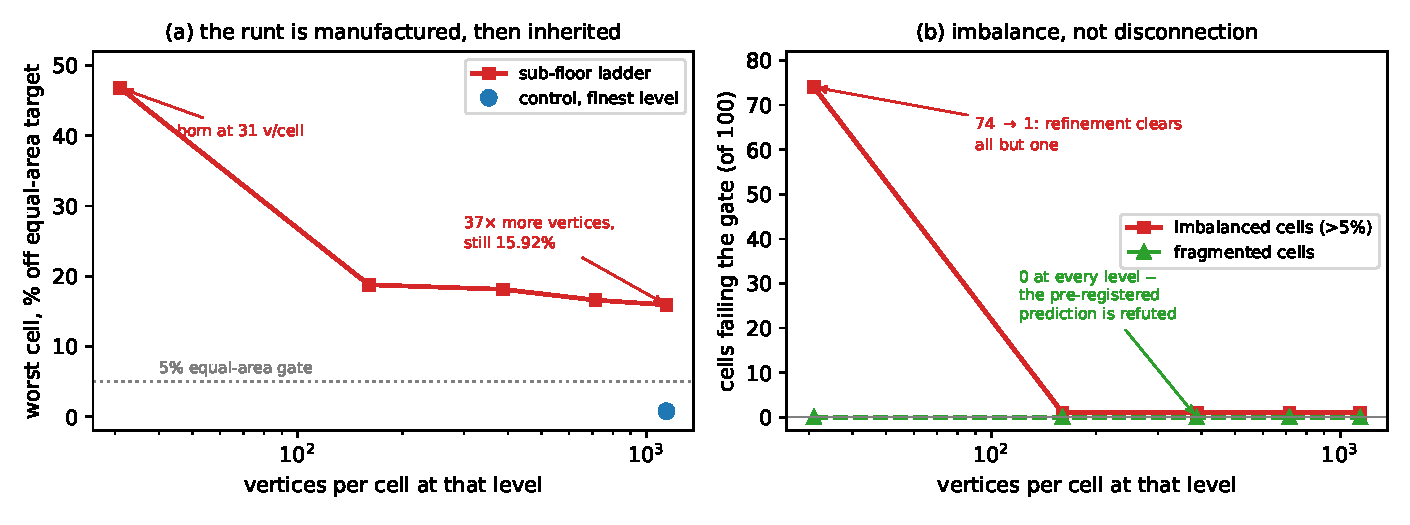
\includegraphics[width=\linewidth]{fig_runt_persistence.pdf}
  \caption{The damage a sub-floor coarsest level leaves behind. (a)~The worst
  cell's discrete-area deviation opens at \(46.80\%\) on the 31 v/cell level and
  is still \(15.92\%\) on the finest mesh, never crossing the \(5\%\) gate,
  against a control that ends at \(0.78\%\) on the identical mesh.
  (b)~Refinement clears 73 of the 74 imbalanced cells but not the last one;
  fragmented cells are 0 at every level.}
  \label{fig:runt}
\end{figure}

The arm is a \emph{gate failure}: 1 of 100 cells over the \(5\%\) threshold,
cell~32 at \(15.92\%\) (absolute \(0.03771\), which is exactly the Phase~2
iteration-0 equal-area constraint violation this solution would hand downstream).

The trajectory is the finding. Between level~1 and level~5 the mesh grows
\(37\times\) --- from 3{,}120 to 114{,}144 vertices, ending at the control's own
finest mesh --- and the worst cell improves only \(46.80\% \to 15.92\%\). It is
still three times over the gate. \textbf{A defect created on a starved coarsest
level is inherited, not healed}, even by a mesh that on the control's ladder
produced \(0.78\%\).

\paragraph{One confound, stated.} The arm sets
\code{struct\_trigger\_enabled: true} and the control does not, so the two differ
in a second knob. It bit level~1 only, stopping it at 3{,}000 iterations
(``structure frozen: 3 label flips over the last 2{,}000''); every other level
ended on the ordinary plateau trigger. This cannot touch Result~1 --- a trigger
that stops a level early cannot \emph{remove} fragmentation that a longer run
would have shown, and there was none at any level --- but it means the
\(15.92\%\) is a mild \emph{upper} bound on how well this ladder could do: an
un-triggered level~1 might have ground the runt down further. It would have to
recover \(11\%\) to reach the gate. The re-based \(N{=}300\) follow-up
(\codefile{parameters/torus\_300part\_rebased\_ladder.yaml}) leaves the trigger
off for exactly this reason.

Two controls on that reading. First, the geometry at large is comparable: the
initial contour-extraction perimeter is \(214.1032\) here against the control's
\(214.3413\) --- \(0.11\%\) apart --- so the harm is concentrated in one cell's
area share, not distributed. Second, the sub-floor ladder is \emph{cheaper}, not
more expensive: \(\sim\!24{,}300\)~s against the control's \(48{,}132\)~s, because
the control's level~0 alone burns 19{,}583~s running to the 30{,}000-iteration
cap. Halving the ladder cost while breaking the partition is precisely the
trade the four prior arms were making, arrived at from the opposite direction.

\section{Result 3 --- ``\code{LINE SEARCH STALLED}'' is normal convergence}
\label{sec:stall}

\begin{figure}[htbp]
  \centering
  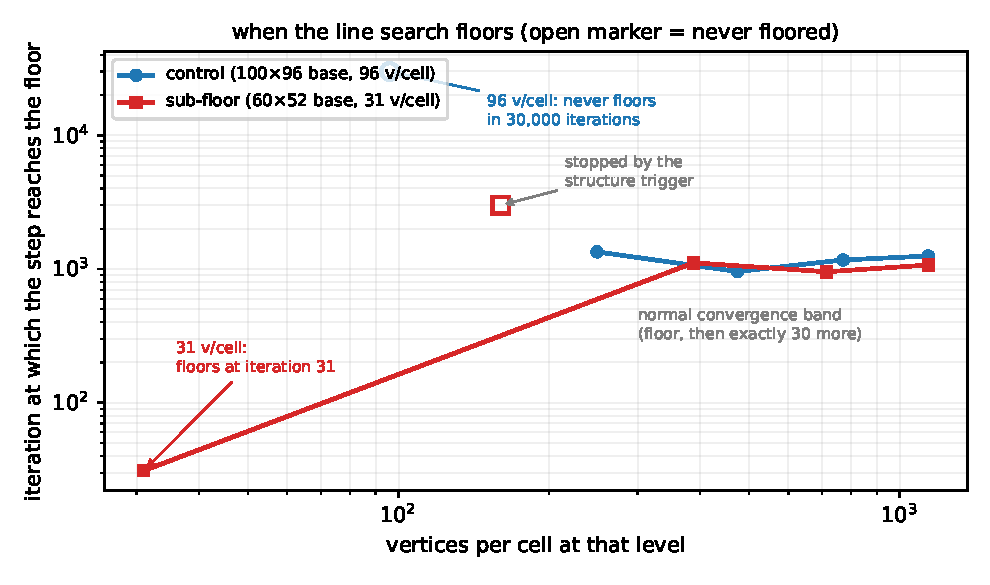
\includegraphics[width=0.82\linewidth]{fig_floor_onset.pdf}
  \caption{When the Armijo step reaches the backtracking floor
  \(9.0949\times10^{-13} = \text{step}_0\rho^{40}\), against vertices per cell.
  Filled markers floored; open markers never did. Every floored level --- in the
  \emph{validated control} as much as in the arm --- then runs exactly
  \code{refine\_patience}\,\(=30\) more iterations before the refinement trigger
  fires.}
  \label{fig:floor}
\end{figure}

The stall guard added in \code{1b2ad04} reports a floored line search as ``a dead
optimizer masquerading as convergence,'' and \code{db737ea} built on it: the
claim that \(N{=}300\)'s two coarsest levels ``provably do not converge --- they
stall at iterations 31 and 41.'' Checking the guard against the control shows
this reading is wrong.

\begin{center}
\small
\begin{tabular}{@{}lrrrrr@{}}
\toprule
 & v/cell & iterations & first floored & trailing floored block & \\
\midrule
\multicolumn{5}{@{}l}{\emph{control} \code{run\_20260709\_081548} --- 0 imbalanced, 0 fragmented} \\
level 0 & 96      & 30{,}000 (cap) & --- & 0  & never floors \\
level 1 & 249     & 1{,}372 & 1{,}343 & \textbf{30} & \\
level 2 & 475     & 986     & 957     & \textbf{30} & \\
level 3 & 772     & 1{,}197 & 1{,}168 & \textbf{30} & \\
level 4 & 1{,}141 & 1{,}279 & 1{,}250 & \textbf{30} & \\
\midrule
\multicolumn{5}{@{}l}{\emph{sub-floor arm}} \\
level 0 & 31      & 60      & \textbf{31} & \textbf{30} & \\
level 1 & 160     & 3{,}000 & --- & 0 & structure trigger \\
level 2 & 388     & 1{,}141 & 1{,}112 & \textbf{30} & \\
level 3 & 715     & 982     & 953     & \textbf{30} & \\
level 4 & 1{,}141 & 1{,}100 & 1{,}071 & \textbf{30} & \\
\bottomrule
\end{tabular}
\end{center}

The trailing block is \textbf{exactly 30} in every floored level of both runs,
and \code{refine\_patience: 30}. The mechanism is plain: PGD reaches an iterate
where no backtracked step satisfies Armijo, the step floors, the energy freezes,
and 30 iterations later the plateau trigger's patience is satisfied and
refinement fires. \emph{That is how a healthy level terminates.} The control's
level~4 ends frozen at \(E{=}92.155173\), \(\|g\|{=}3.1609\); the arm's ends at
\(E{=}94.160421\), \(\|g\|{=}3.1740\). Same behaviour, and one of them is the
validated deliverable.

Three consequences.

\begin{enumerate}
  \item \textbf{The guard fires on every healthy level termination.}
    \code{\_warn\_if\_stalled} triggers when any step was rejected in the run-up
    to the trigger --- but the patience window \emph{is} 30 rejected iterations by
    construction, so the condition holds identically on good and bad runs. It was
    calibrated on the A2 arm, where flooring genuinely was pathological
    (\codefile{docs/experiments/05-soft-area-constraint/} \S Result~3), but the
    terminal signature is the same on the exact path, so it cannot discriminate.
  \item \textbf{Only the \emph{timing} of the floor is diagnostic, and it is
    strongly resolution-dependent.} Figure~\ref{fig:floor}: a cold level~0 at
    31 v/cell floors at iteration \textbf{31}; the same cold level~0 at
    96 v/cell never floors across 30{,}000 iterations; warm-started levels at
    \(\geq\!388\) v/cell floor at \(\sim\!950\text{--}1{,}250\). The
    \(N{=}300\) level-0 figure this experiment set out to explain --- ``stalls
    at 31'' at 32 v/cell --- is reproduced here almost exactly at 31 v/cell.
    That reproduction stands; the interpretation of it as ``does not converge''
    does not.
  \item \textbf{Stage~2's refutation criterion was unusable as written.} It said
    a stall \emph{above} the floor would refute the hypothesis --- but the control
    stalls above the floor on four levels, as does this arm's own level~4 at
    1{,}141 v/cell.
\end{enumerate}

\subsection{The fix}
\label{sec:stall-fix}

The guard is retained but re-based on \emph{onset}: it fires only when the step
reaches the floor inside the first \code{\_STALL\_EARLY\_ITERS} (200) iterations
of a level, and is silent otherwise, because flooding later is convergence. A
ratio of the level's own length would not work --- a starved level floors early
\emph{and} terminates early, so 31 of 60 iterations is \(51.7\%\), not a small
fraction --- so the test is against an absolute iteration count. The margin above
200 is \(\mathbf{1.13\times}\): the earliest floor among levels the rule leaves
silent is iteration \textbf{227}. This paragraph originally claimed
\(6.7\times\), computed from the control's own level~1 at 1{,}343 --- a figure
that contradicted this report's own table two paragraphs below (314) even before
the corpus was corrected. See the correction after the replay table. The message
is renamed from \code{LINE SEARCH STALLED} to \code{UNDER-RESOLVED LEVEL} and now
says what to do about it.

\subsubsection*{Replay validation}

The rule was replayed offline over the STEP column of 130 PGD summary traces
across 40 runs, \(N{=}10\) to \(N{=}300\). Of these, 24 fire and 106 are silent
(24 of the silent never floored at all). The threshold is not a tuned parameter:
it falls in an empty gap --- \emph{narrower} than this section first reported.

\begin{center}
\small
\begin{tabular}{@{}lrr@{}}
\toprule
 & levels & first floored iteration \\
\midrule
fires (onset \(<200\))        & 24  & 18 -- \textbf{100} \\
\emph{(replayed subset: none; full tree: 3)} & 0 & 101 -- 313 \\
silent, floored later         & 82  & \textbf{314} -- 22{,}574 \\
silent, never floored         & 24  & --- \\
\bottomrule
\end{tabular}
\end{center}

\begin{tcolorbox}[colback=red!4!white,colframe=red!55!black,
  title={Correction (2026-08-15, adversarial review): the replay corpus was a
  subset, and the gap is narrower}]
This section originally described the corpus as \emph{``every PGD summary trace
in} \code{results/}\emph{''}. It is not. \code{results/} holds \textbf{350}
summary traces; the replay's glob (\code{results/run\_*/traces/}) could only ever
reach the top-level run directories, leaving \textbf{185} traces in the sweep
directories structurally invisible, plus \(\sim\!35\) double-torus / Banchoff runs
whose \code{v1ngx}-style filenames the parsing regex could not read. The 130/40
figures describe torus \(+\) ellipsoid top-level runs only.

On the full tree, three \code{torus\_npart10} sweep levels floor at \textbf{227,
280 and 303} --- inside the range this section called empty. Therefore:

\begin{itemize}\itemsep2pt
  \item the real empty gap is \((100,\,227)\), not \((100,\,314)\);
  \item ``anything from 101 to 313 would give the same verdict'' is
    \textbf{false} --- a threshold of \textbf{250 would misfire};
  \item the margin above 200 is \(\mathbf{1.13\times}\), not \(6.7\times\).
\end{itemize}

\textbf{The guard's verdicts are unaffected}: nothing in \code{results/} floors in
\([100,\,226]\), so \code{\_STALL\_EARLY\_ITERS} \(=200\) classifies all 350
levels exactly as intended. What was wrong is the advertised robustness --- and
the error is the same class this report warns about elsewhere: a corpus whose
construction guaranteed the pattern it was then cited to prove.
\end{tcolorbox}

All five levels of the validated control are silent, including its level~0 at
96 v/cell. The levels that fire are \(N{=}300\)'s levels 0 and 1, \(N{=}200\)'s
level 0 (48 v/cell, floor at 21--27), \(N{=}150\)'s level 0 (64 v/cell, floor at
47), and this arm's level 0 --- but see the boundary correction in
\S\ref{sec:scaling}: this list is \emph{not} evidence that ``every level below
\(\sim\!90\) v/cell fires'', since \code{run\_20260629\_141012} fires at 96
v/cell.

Two things the replay shows that the resolution framing alone does not.
\textbf{Low resolution is the usual cause but not the only one}: the known-bad
\(N{=}100\) \(\lambda{=}2.1\) run \code{run\_20260701\_143238} fires at 193 and
501 v/cell, correctly --- those levels did die at iterations 47 and 100, and that
config is documented as outside the \(\lambda\) working window. So the guard
reads ``this level died before doing any work,'' with resolution the first thing
to check and \code{lambda\_penalty} the second; the warning text says both.
\textbf{And it catches the adaptive soft-area arm}: \code{run\_20260813\_003231}
level~3, at 257 v/cell --- above the floor --- floors at iteration 23, which is
the soft treatment's line-search collapse of report~05, not a resolution
problem.

Finally, an honest limit: this rule does \emph{not} detect the A2 pathology
where every level floored \emph{late} and the collapse was still real. Late
collapse needs a different signal, and none is proposed here.

\section{What this means for scaling}
\label{sec:scaling}

\subsection{Which threshold this report measured}

It is \emph{not} the \(\sim\!250\text{--}300\) v/cell \emph{gate} floor of
\codefile{docs/reference/winner\_take\_all\_partition\_gap.md} \S4b --- the
resolution at which a level can itself drive the worst cell under the \(5\%\)
gate. What the sub-floor arm crossed is a much lower and much sharper boundary:
whether the level \emph{runs at all}. From the replay of \S\ref{sec:stall}, by
vertices per cell:

\begin{center}
\small
\begin{tabular}{@{}lll@{}}
\toprule
v/cell & iterations before the step floors & \\
\midrule
31, 32, 48, 64, 83 & 18--47 & \textbf{dies} \\
92, 96 & 1{,}141, or never in 30{,}000 & \textbf{runs} \\
\bottomrule
\end{tabular}
\end{center}

The mechanism is not ``a coarse level does bad work'' but ``a coarse level does
\emph{no} work'': it dies in tens of iterations, the cheap equalization phase
never happens there, and the first level that does run starts from a badly
imbalanced field instead of from a nearly balanced one. That is exactly the arm
measured here --- the control's level~0 at 96 v/cell runs 30{,}000 iterations and
equalizes from the seeded init; the arm's at 31 v/cell dies at iteration~31.

\begin{tcolorbox}[colback=red!4!white,colframe=red!55!black,
  title={Correction (2026-08-15, adversarial review): the boundary's
  \emph{location} is not established}]
This subsection originally concluded ``the boundary sits between 83 and 92
v/cell.'' That is \textbf{refuted as stated}, and the table above must be read as
a list of onsets rather than as a threshold.

\begin{itemize}\itemsep2pt
  \item The row ``92, 96 \(\to\) runs'' is false. \code{run\_20260629\_141012} is
    \textbf{96 v/cell and floors at onset 32} --- and it was present, unremarked,
    in this very replay's own fire-list. Its \(\lambda{=}2.1\) is below the
    \(N{=}100\) working window. Also observed but omitted: 96 v/cell flooring at
    2{,}202 and 92 v/cell at 5{,}247.
  \item Verts-per-cell is causally implicated by exactly \textbf{one controlled
    pair} --- the sub-floor arm of this report (\(N{=}100\), \(\lambda{=}5.1\):
    31 dies at 30, 96 never floors). Everything else pooled into ``83--92''
    varies in \(\lambda\)-window membership and straddles the 2026-07-06 energy
    fix, and the dies-set silently drops \(\lambda\)/arm pathologies at
    158/193/237/249/257/501 v/cell.
  \item Cold-vs-warm start was suspected as the confound and is \textbf{refuted}
    (the dies-set contains warm 83 v/cell levels; the runs-set at 92/96 is cold).
    Separated by start type the brackets are cold \((64, 92)\) and warm
    \((83, 124)\) --- wide and overlapping.
\end{itemize}

What survives is the \emph{mechanism} (a level can die doing no work, and the
damage is inherited) and the one controlled pair. The \emph{number} does not, so
the \(N{=}1000\) mesh-budget arithmetic in \S\ref{sec:scaling} and the dismissal
of \codefile{parameters/torus\_300part\_rebased\_ladder.yaml} at 51 v/cell both
inherit this uncertainty.
\end{tcolorbox}

\subsection{Cross-check at \texorpdfstring{\(N{=}300\)}{N=300}}

The same quantities were reconstructed for free from the \(\lambda{=}11.5\)
\(N{=}300\) control's saved trace iterates (its \code{traces/*\_internal\_data.hdf5}
store \code{x}; rebuild each level's mesh and run the gates):

\begin{center}
\small
\begin{tabular}{@{}lrrrrl@{}}
\toprule
stage & mesh & v/cell & imbalanced & worst \% & estimator \\
\midrule
seeded init & --- & --- & 230 & 44.02 & exact \\
after L0 & 100\(\times\)96  & 32  & 234 & 45.57 & L1 \code{iter\_0} proxy \\
after L1 & 162\(\times\)154 & 83  & 234 & 49.26 & L2 \code{iter\_0} proxy \\
after L2 & 224\(\times\)212 & 158 & 10  & 36.15 & true final \\
after L3 & 286\(\times\)270 & 257 & 4   & 27.04 & same-level iter\_3500 \\
after L4 & 348\(\times\)328 & 380 & 3   & 24.81 & true final \\
\bottomrule
\end{tabular}
\end{center}

Both of \(N{=}300\)'s coarse levels die, handing forward what the init gave them
(230 \(\to\) 234). The equalization therefore happens at level~2 (158 v/cell),
and levels 3--4 then improve with decelerating returns. So the same mechanism
this report measures at \(N{=}100\) is visibly present at \(N{=}300\).

\begin{tcolorbox}[colback=red!4!white,colframe=red!55!black,
  title={Correction (2026-08-15, adversarial review): mixed estimators, and
  level~2 did not demonstrably converge}]
\begin{enumerate}[leftmargin=*,itemsep=3pt]
  \item \textbf{The \code{estimator} column is new, and the table needs it.} Three
    different meanings of ``after level L'' were pooled undisclosed. At the one
    junction where both sides exist (end-L2 \(\to\) L3 \code{iter\_0}), mesh
    resampling \textbf{triples} the imbalanced count, \(10 \to 31\), and changes
    the worst cell's identity (299 \(\to\) 290); worst \% is robust
    (36.15 \(\to\) 35.69). L4's actual \code{iter\_0} is \textbf{6 cells /
    25.94\%}, not the 4 / 27.04 tabled.
  \item \textbf{The coarse rows are unharmed, and stronger than written.}
    Interpolating and projecting the seeded init reproduces L1's \code{iter\_0}
    labels \textbf{100.000\%} (0 of 24{,}948 differ) --- so L0's 47 iterations
    flipped \emph{zero} argmax labels, and the \(+4\) is pure resampling.
  \item \textbf{``Converges there'' is withdrawn.} The flatness is real and exact
    (36.149069\% to six decimals at iters 6000/6500/final), but the flat window is
    \(\sim\!658\) iterations, not 1{,}000 (iter 5500 = 36.47\%), and the
    termination shows the opposite of convergence: the line search
    \textbf{floored at 6{,}628 with the energy still falling} (\(-0.667\) over the
    last 1{,}000 pre-floor) and \(\|g\| = 31.11\). By this report's own
    \S\ref{sec:stall}, flooring certifies nothing in either direction --- and that
    cuts against ``converged'' exactly as it cut against ``failed''.
  \item \textbf{The gains are partly resampling.} L4's \(-2.23\) pts is
    \(-1.13\) optimization \(+\) \(-1.10\) resampling; L3's \(-9.11\) is
    \(-8.65 + -0.46\).
\end{enumerate}
Conclusions in \S\ref{sec:conclusions} survive, but any claim that \(N{=}300\) is
\emph{energy-limited} rather than descent-limited is unsupported by these data.
\end{tcolorbox}

\subsection{What does not follow}

Two limits on how far to push this, both important.

\textbf{The floor is cheap, not expensive.} An earlier draft of this section put
the fix at \(V \propto N\) with \(\sim\!250\text{--}300\) v/cell at every level,
which at \(N{=}1000\) would demand a \emph{coarsest} level of
\(V \approx 250\text{--}300\)k. That inherited the wrong threshold. At the
measured \(\sim\!90\) v/cell boundary the coarsest level at \(N{=}1000\) is
\(V \approx 90\)k --- a factor of 3 smaller, and unremarkable next to the finest
meshes already run here.

\textbf{A dying level~0 is not by itself fatal.} \(N{=}200\) reaches 0
imbalanced (worst \(1.65\%\)) with a level~0 at 48 v/cell that also dies at
iteration 21 --- because its \emph{level 1}, at 124 v/cell, runs 12{,}155
iterations and does the equalization there. The requirement that fits every run
measured is therefore weaker and less tidy than ``level 0 must clear a
threshold'': \emph{some early, cheap level must run long enough to equalize
before the expensive levels begin.} \(N{=}100\) gets one at level 0,
\(N{=}200\) at level 1, and \(N{=}300\)'s first is level 2 at 158 v/cell running
6{,}658 iterations --- later, and less than half as long.

Whether giving \(N{=}300\) an earlier, longer-running equalization level would
move its converged answer is \textbf{untested}. This report shows the converged
point \emph{is} start-dependent --- identical finest mesh, \(0.78\%\) vs
\(15.92\%\) --- which makes the question worth asking; it does not answer it.
Note the naive version of that test is not the one to run:
\codefile{parameters/torus\_300part\_rebased\_ladder.yaml} lifts level~0 only to
51 v/cell, still inside the dying regime.

\section{Conclusions}
\label{sec:conclusions}

\begin{enumerate}
  \item \textbf{The hypothesis is refuted on its stated terms.} A sub-floor
    coarsest level does not manufacture disconnected cells at \(N{=}100\): 0
    fragmented at all five levels. \(N{=}300\)'s cells 274 and 290 have another
    cause, and Stage~2 should not be run. This cost 6.8~h instead of the several
    days a direct \(N{=}300\) test would have.
  \item \textbf{It is confirmed on an axis it did not pre-register.} A starved
    level~0 manufactures a runt that survives \(37\times\) refinement onto the
    control's own finest mesh: \(46.80\% \to 15.92\%\), still three times over
    the gate, against \(0.78\%\). Damage at level~0 is inherited.
  \item \textbf{A pre-registered experiment can be refuted and still pay.} The
    fragmentation prediction failed; the run nonetheless produced the first
    controlled measurement of what the resolution floor is worth, and it did so
    by changing exactly one variable against a known-good control.
  \item \textbf{Check a new diagnostic against a known-good run before building
    on it.} The stall guard was calibrated on a failing arm and never run against
    the validated control, where it fires on four of five levels. Two commits
    reasoned from it. A guard that has only ever seen sick patients cannot tell
    you what healthy looks like.
  \item \textbf{Cheapness was never the broken axis.} The sub-floor ladder is
    half the control's wall time and produces an invalid partition. Any future
    arm should be judged on validity per unit compute, not on either alone.
\end{enumerate}

\section*{Related documents}
\addcontentsline{toc}{section}{Related documents}

\begin{itemize}
  \item \codefile{docs/reference/winner\_take\_all\_partition\_gap.md} --- the
    standing explanation; \S4b states the resolution floor this report measures,
    \S4c the locality criterion.
  \item \codefile{docs/plans/PHASE1\_N1000\_VALIDITY\_PLAN.md} --- P3
    (mesh-budget validity floor) is the proposal this report supplies evidence
    for.
  \item \codefile{docs/experiments/05-soft-area-constraint/} --- the arm the
    stall guard was written for, and where flooring genuinely was pathological.
  \item \codefile{docs/experiments/04-territory-aware-highn-validation/} --- the
    other cheapening arm that failed on connectivity.
  \item Configs: \codefile{parameters/torus\_100part\_subfloor\_ladder.yaml}
    (this run), \codefile{parameters/torus\_300part\_above\_floor\_ladder.yaml}
    (Stage~2, \emph{not} run --- gate failed).
  \item Code: \codefile{src/optimization/pgd\_optimizer.py} (stall guard),
    \codefile{testing/watch\_level\_gates.py} (per-level gates).
\end{itemize}

\end{document}
